\chapter{Descrição do Experimento}

Este capítulo apresenta uma descrição detalhada do ambiente experimental utilizado para validação da proposta, incluindo a configuração do ambiente de testes, a definição dos módulos principais e auxiliares do sistema, os detalhes de implementação de cada componente, o processo de geração de conteúdo multimídia e, por fim, a especificação dos cenários de teste utilizados para a análise comparativa dos algoritmos de balanceamento de carga.

\section{Ambiente de Experimentação}

O ambiente experimental foi configurado para proporcionar um cenário controlado e reproduzível, capaz de simular condições realistas de operação de um sistema de distribuição de conteúdo. A infraestrutura foi estabelecida em uma única máquina física operando o sistema operacional Windows, com o subsistema Windows para Linux (WSL2) configurado para execução de um \textit{kernel} Linux completo. Esta escolha arquitetural permite a utilização de recursos nativos do Linux, como o sistema de grupos de controle (\textit{cgroups}), essenciais para o monitoramento e limitação de recursos computacionais dos contêineres.

A plataforma de conteinerização Docker foi empregada como ambiente de execução para todos os componentes do sistema. O Docker oferece isolamento de processos, gerenciamento de recursos e padronização do ambiente de execução, garantindo que os experimentos possam ser reproduzidos de forma consistente. Além disso, a utilização de contêineres elimina problemas relacionados a dependências de bibliotecas e configurações de sistema operacional, assegurando que cada componente opere em um ambiente idêntico e controlado.

\subsection{Particularidades do Docker e cgroups}

O Docker utiliza o sistema de \textit{cgroups} (grupos de controle) do kernel Linux para implementar limites de recursos e realizar o monitoramento de uso de CPU, memória e entrada/saída de disco. Especificamente, o experimento utiliza \textit{cgroups v2}, que oferece uma interface unificada e simplificada para o gerenciamento de recursos. Através dos arquivos de sistema disponibilizados pelo \textit{cgroups}, é possível ler diretamente as métricas de consumo de memória e taxa de leitura de disco de cada contêiner em tempo real.

Para garantir a consistência entre as execuções dos experimentos e eliminar o efeito de \textit{cache} do sistema operacional nos resultados, é fundamental realizar a limpeza do \textit{cache} de páginas do kernel Linux antes de cada execução. Esta operação é realizada através do comando:

\begin{verbatim}
echo 3 | sudo tee /proc/sys/vm/drop_caches
\end{verbatim}

Este comando instrui o kernel a liberar os \textit{caches} de página (\textit{pagecache}), \textit{dentries} e \textit{inodes}, garantindo que cada execução do experimento parta de um estado limpo, sem dados previamente armazenados em memória. A operação requer privilégios de superusuário (\texttt{sudo}) e é executada antes de cada bateria de testes.

O Docker também permite a configuração de limites explícitos de recursos para cada contêiner através de parâmetros na configuração do \textit{Docker Compose}. No experimento, foram configurados limites de memória RAM (através do parâmetro \texttt{memory}) e limites de taxa de leitura de disco (através do parâmetro \texttt{device\_read\_bps}). Estes limites são fundamentais para simular servidores com capacidades heterogêneas, permitindo avaliar o comportamento do algoritmo de balanceamento em cenários com recursos desiguais.

\subsection{Organização do conteúdo e bind mounts}

Para simular o cenário realista de servidores de distribuição de conteúdo com arquivos exclusivos, foi necessário replicar o conteúdo de vídeo em múltiplos diretórios no sistema de arquivos do host WSL. O conteúdo multimídia foi armazenado em um diretório global localizado em \texttt{/data} no sistema de arquivos Linux do WSL, com subdiretórios específicos para cada servidor (\texttt{/data/server-1}, \texttt{/data/server-2}, e assim por diante até \texttt{/data/server-8}).

Cada contêiner de servidor MPEG-DASH foi configurado com um \textit{bind mount} que mapeia o diretório específico do servidor no host para o diretório interno do contêiner. Esta técnica permite que cada servidor acesse apenas seu próprio conjunto de arquivos, simulando a exclusividade de conteúdo encontrada em servidores de borda de uma CDN real. O uso de \textit{bind mounts} também evita a necessidade de copiar os arquivos para dentro das imagens Docker, reduzindo o tamanho das imagens e facilitando a atualização do conteúdo sem reconstruir os contêineres.

\section{Definição dos Módulos}

O sistema experimental é composto por módulos principais e auxiliares, cada um desempenhando uma função específica na arquitetura do experimento. Esta seção descreve a organização e o propósito de cada componente.

\subsection{Módulos Principais}

Os módulos principais formam o núcleo funcional do sistema de distribuição de conteúdo e são responsáveis pelo processamento e encaminhamento das requisições dos clientes:

\begin{enumerate}
    \item \textbf{Servidores MPEG-DASH}: Conjunto de 8 instâncias de servidores web responsáveis por servir o conteúdo de vídeo segmentado de acordo com o padrão MPEG-DASH. Cada servidor é executado em um contêiner Docker isolado e possui limites específicos de memória e taxa de leitura de disco, permitindo a simulação de servidores com capacidades heterogêneas. Os servidores também são responsáveis por coletar e publicar suas próprias métricas de consumo de recursos.
    
    \item \textbf{Balanceador de Carga}: Componente central do experimento, responsável por receber todas as requisições HTTP dos clientes e distribuí-las entre os servidores MPEG-DASH disponíveis de acordo com a estratégia de balanceamento configurada. O balanceador opera como um \textit{proxy} reverso HTTP e é implementado para suportar múltiplas estratégias de seleção de servidor, permitindo a comparação entre diferentes algoritmos.
    
    \item \textbf{Gerador de Carga}: Aplicação cliente que simula múltiplos usuários acessando o sistema de forma concorrente. O gerador é parametrizável em termos de número de usuários simultâneos e duração do teste, permitindo a criação de cenários de carga variados para avaliar o comportamento do sistema sob diferentes níveis de estresse.
\end{enumerate}

\subsection{Módulos Auxiliares}

Os módulos auxiliares fornecem serviços de suporte necessários para o funcionamento e monitoramento do sistema:

\begin{enumerate}
    \item \textbf{\textit{Broker} MQTT (NanoMQ)}: Serviço de mensageria que implementa o protocolo MQTT (\textit{Message Queuing Telemetry Transport}), um protocolo leve de comunicação \textit{publish-subscribe}. O \textit{broker} atua como intermediário, recebendo as métricas publicadas pelos servidores MPEG-DASH e disponibilizando-as para o balanceador de carga através de assinaturas em tópicos específicos. O uso do MQTT permite a comunicação assíncrona e desacoplada entre os componentes.
    
    \item \textbf{Painel de Monitoramento em Tempo Real}: Interface web que oferece visualização gráfica e em tempo real das métricas de cada servidor e do balanceador de carga. O painel permite acompanhar o comportamento do sistema durante os experimentos, facilitando a detecção de anomalias e a compreensão do comportamento dinâmico do algoritmo de balanceamento.
    
    \item \textbf{Coletor de Métricas (API)}: Serviço Python que expõe uma API REST para consulta das métricas dos contêineres através do acesso direto aos arquivos do \textit{cgroups}. Este componente complementa o monitoramento realizado internamente pelos servidores, permitindo a validação cruzada das métricas e fornecendo dados para o painel de monitoramento.
\end{enumerate}

\section{Detalhes de Implementação dos Módulos}

Esta seção apresenta os detalhes técnicos de implementação de cada módulo do sistema, incluindo as tecnologias empregadas, as principais funcionalidades e os trechos de código mais relevantes.

\subsection{Servidores MPEG-DASH}

Os servidores MPEG-DASH foram implementados utilizando ASP.NET Core 8.0, uma plataforma de desenvolvimento web moderna e de alto desempenho da Microsoft. A escolha desta tecnologia foi motivada por sua capacidade nativa de servir arquivos estáticos de forma eficiente, sua arquitetura assíncrona que permite alto nível de concorrência e a disponibilidade de bibliotecas para comunicação MQTT.

Cada servidor é configurado como uma aplicação web mínima que serve arquivos estáticos do diretório \texttt{wwwroot/Static}, onde estão armazenados os segmentos de vídeo MPEG-DASH. A aplicação não realiza processamento de vídeo em tempo real; ela apenas entrega os arquivos pré-processados aos clientes que os solicitam.

\subsubsection{Monitoramento e Publicação de Métricas}

O componente mais crítico da implementação dos servidores é o sistema de monitoramento de recursos e publicação de métricas. Esta funcionalidade é implementada através da classe \texttt{MetricsPublisher}, um serviço de segundo plano (\textit{background service}) que executa continuamente enquanto o servidor está ativo.

O \texttt{MetricsPublisher} realiza periodicamente as seguintes operações:

\begin{enumerate}
    \item Leitura do consumo atual de memória através do arquivo \texttt{/sys/fs/cgroup/memory.current} do \textit{cgroups v2};
    \item Leitura das estatísticas de entrada/saída através do arquivo \texttt{/sys/fs/cgroup/io.stat}, extraindo o total de \textit{bytes} lidos (\texttt{rbytes});
    \item Cálculo da taxa de leitura de disco através da diferença entre leituras consecutivas dividida pelo intervalo de tempo decorrido;
    \item Normalização das métricas em relação aos limites configurados para o contêiner, gerando valores entre 0 e 1;
    \item Publicação das métricas normalizadas em um tópico MQTT para consumo pelo balanceador de carga.
\end{enumerate}

O intervalo de publicação é configurável através da variável de ambiente \texttt{METRICS\_PUBLISH\_INTERVAL\_SECONDS}, permitindo avaliar o impacto da frequência de atualização das métricas no desempenho do algoritmo de balanceamento.

A estrutura de dados publicada contém os seguintes campos:

\begin{itemize}
    \item \texttt{memory\_current}: Consumo normalizado de memória (0 a 1);
    \item \texttt{disk\_read}: Taxa normalizada de leitura de disco (0 a 1);
    \item \texttt{active\_request\_count}: Número de requisições HTTP ativas sendo processadas no momento;
    \item \texttt{timestamp\_unix}: \textit{Timestamp} Unix da coleta.
\end{itemize}

O contador de requisições ativas é implementado através da classe \texttt{RequestCounter}, que utiliza operações atômicas para incrementar e decrementar o contador de forma \textit{thread-safe}, garantindo a consistência dos dados mesmo sob alta concorrência.

\subsection{Balanceador de Carga}

O balanceador de carga foi implementado em Rust, uma linguagem de programação de sistemas que oferece garantias de segurança de memória em tempo de compilação e desempenho comparável a linguagens como C e C++. A escolha do Rust foi motivada pela necessidade de alto desempenho e baixa latência no processamento das requisições, características essenciais para um componente crítico como o balanceador de carga.

\subsubsection{Arquitetura e Funcionamento}

O balanceador opera como um \textit{proxy} reverso HTTP, recebendo requisições dos clientes na porta 8080 e encaminhando-as para um dos servidores MPEG-DASH disponíveis. Um aspecto fundamental da implementação é que o balanceamento ocorre ao nível de cada requisição HTTP individual. Isso significa que, durante uma única sessão de reprodução MPEG-DASH, diferentes requisições (como a solicitação do manifesto MPD, dos segmentos de inicialização e dos segmentos de mídia) podem ser atendidas por servidores diferentes, dependendo das decisões tomadas pelo algoritmo de balanceamento a cada momento.

A arquitetura do balanceador é baseada no padrão de projeto \textit{Strategy}, que permite a fácil substituição do algoritmo de seleção de servidor sem modificar o código principal do balanceador. O \textit{trait} \texttt{ServerSelectionStrategy} define a interface que deve ser implementada por qualquer estratégia de balanceamento:

\begin{verbatim}
pub trait ServerSelectionStrategy: Send + Sync {
    fn pick_server(&self, servers: &[String]) -> Option<String>;
}
\end{verbatim}

Esta abstração permite que o experimento compare diferentes algoritmos de balanceamento utilizando exatamente a mesma infraestrutura, garantindo que as diferenças observadas nos resultados sejam devidas exclusivamente ao algoritmo e não a variações na implementação.

\subsubsection{Estratégias de Balanceamento Implementadas}

Três estratégias de balanceamento foram implementadas para fins de comparação:

\begin{enumerate}
    \item \textbf{Round-Robin}: Estratégia determinística que seleciona os servidores de forma cíclica, garantindo uma distribuição uniforme das requisições ao longo do tempo. A implementação utiliza um contador atômico que é incrementado a cada seleção.
    
    \item \textbf{Seleção Aleatória}: Estratégia não-determinística que seleciona um servidor de forma uniformemente aleatória entre os disponíveis. Esta estratégia serve como linha de base para avaliar o ganho proporcionado por estratégias mais sofisticadas.
    
    \item \textbf{Monitoramento de Memória}: Estratégia proposta neste trabalho, que utiliza as métricas de consumo de memória e disco publicadas pelos servidores para calcular probabilidades de seleção baseadas na carga atual e na interpretação de dados potencialmente obsoletos, conforme descrito no Capítulo 3.
\end{enumerate}

A estratégia de monitoramento de memória mantém uma estrutura de dados interna com as métricas mais recentes de cada servidor, que é atualizada através de uma assinatura MQTT no tópico \texttt{loadbalancer/metrics}. Quando uma nova requisição chega, o algoritmo calcula as probabilidades de seleção de acordo com as Equações \ref{eq:basic_li} e \ref{eq:limemory}, e realiza uma seleção aleatória ponderada baseada nessas probabilidades.

\subsection{Gerador de Carga}

O gerador de carga é uma aplicação Python que utiliza a biblioteca \texttt{aiohttp} para realizar requisições HTTP assíncronas de alto desempenho. A implementação é baseada em um modelo de concorrência com múltiplas \textit{coroutines} assíncronas (\textit{workers}), onde cada \textit{worker} simula o comportamento de um cliente MPEG-DASH real.

\subsubsection{Simulação de Clientes MPEG-DASH}

Cada \textit{worker} do gerador de carga executa o seguinte fluxo de operações, que emula o comportamento de um \textit{player} de vídeo MPEG-DASH:

\begin{enumerate}
    \item \textbf{Seleção de Conteúdo}: O \textit{worker} seleciona aleatoriamente um dos diretórios de vídeo disponíveis (de \texttt{video-1} até \texttt{video-4}, de acordo com a configuração).
    
    \item \textbf{Requisição do Manifesto MPD}: A primeira requisição HTTP é feita para obter o arquivo MPD (\textit{Media Presentation Description}), que é um documento XML contendo metadados sobre o vídeo, incluindo as resoluções disponíveis, os \textit{bitrates}, a duração dos segmentos e os \textit{templates} de URL para acessar cada segmento.
    
    \item \textbf{\textit{Parsing} do Manifesto}: O arquivo MPD é analisado utilizando a biblioteca padrão \texttt{xml.etree.ElementTree}, extraindo as informações sobre os segmentos de inicialização e os segmentos de mídia de todas as representações (resoluções) disponíveis.
    
    \item \textbf{Requisição dos Segmentos de Inicialização}: Para cada representação (resolução) do vídeo, o \textit{worker} solicita o segmento de inicialização correspondente, que contém informações de \textit{codec} e configuração necessárias para decodificar os segmentos subsequentes.
    
    \item \textbf{Requisição Sequencial dos Segmentos de Mídia}: O \textit{worker} então solicita sequencialmente os segmentos de mídia, aguardando a conclusão de cada requisição HTTP antes de iniciar a próxima. Este comportamento, sem \textit{buffering} antecipado, simula um cenário onde o cliente consome o conteúdo em tempo real, sem realizar \textit{download} prévio de múltiplos segmentos. Esta é uma simulação simplificada que não representa exatamente o comportamento de \textit{players} MPEG-DASH modernos, que geralmente implementam estratégias de \textit{buffering} e seleção adaptativa de qualidade, mas é adequada para gerar carga no sistema e avaliar o desempenho do balanceador.
\end{enumerate}

O número de \textit{workers} concorrentes é parametrizável através do argumento de linha de comando \texttt{--concurrent}, permitindo simular desde cenários de baixa carga (dezenas de usuários) até cenários de alta carga (milhares de usuários simultâneos). A duração do teste também é configurável através do parâmetro \texttt{--duration}, permitindo controlar o tempo total de execução do experimento.

\subsubsection{Aplicação Cliente para Validação e Visualização}

Além do gerador de carga automatizado, foi desenvolvida uma aplicação cliente baseada em HTML (\texttt{test-dash.html}) que utiliza a biblioteca \texttt{dash.js} para reprodução real de vídeos MPEG-DASH com visualização em tempo real das métricas de QoE. Esta aplicação serve como ferramenta de validação e depuração, permitindo observar o comportamento do sistema durante a reprodução de vídeo e coletar dados detalhados sobre a qualidade da experiência do usuário.

A aplicação implementa um \textit{player} de vídeo completo com as seguintes funcionalidades:

\begin{enumerate}
    \item \textbf{Gerenciamento de Sessão de Vídeo}: A aplicação inicializa o \textit{player} \texttt{dash.js} com configurações específicas de \textit{buffer} (\texttt{stableBufferTime}, \texttt{initialBufferLevel}) e registra \textit{handlers} para eventos de reprodução (\texttt{PLAYBACK\_STARTED}, \texttt{PLAYBACK\_WAITING}, \texttt{PLAYBACK\_PLAYING}, \texttt{PLAYBACK\_ENDED}). Esses eventos permitem rastrear o ciclo de vida completo da sessão de reprodução, incluindo o início do \textit{streaming}, momentos de travamento (\textit{stalls}), retomada da reprodução e finalização do vídeo.
    
    \item \textbf{Visualização em Tempo Real}: Três gráficos interativos são atualizados dinamicamente durante a reprodução do vídeo, utilizando a biblioteca \texttt{Chart.js}:
    \begin{itemize}
        \item \textbf{Gráfico de Qualidade (\textit{Quality Timeline})}: Exibe a evolução da qualidade (resolução e \textit{bitrate}) selecionada pelo algoritmo de adaptação do \texttt{dash.js} ao longo dos segmentos de vídeo reproduzidos. O eixo Y representa as diferentes resoluções disponíveis (144P a 1080P), e o eixo X representa a sequência de segmentos, permitindo visualizar as mudanças de qualidade durante a sessão.
        
        \item \textbf{Gráfico de \textit{Bitrate} (\textit{Bitrate Timeline})}: Mostra a taxa de transferência média (\textit{throughput}) medida pelo \texttt{dash.js} para cada segmento baixado, em kilobits por segundo (kbps). Este gráfico utiliza uma escala logarítmica no eixo Y para melhor visualização da variação de \textit{bitrate} ao longo do tempo.
        
        \item \textbf{Gráfico de Travamentos (\textit{Stall Timeline})}: Apresenta um gráfico de dispersão onde cada ponto representa um evento de travamento (\textit{stall}), com a posição no eixo X indicando o segmento onde ocorreu o travamento e o eixo Y mostrando a duração do travamento em segundos. Este gráfico permite identificar visualmente a frequência e a severidade dos travamentos durante a sessão.
    \end{itemize}
    
    \item \textbf{Coleta de Dados para Análise}: Ao final de cada sessão de reprodução, a aplicação exporta automaticamente para o console do navegador arrays estruturados contendo todos os dados coletados:
    \begin{itemize}
        \item Sequência de qualidades reproduzidas (IDs de representação e \textit{labels} descritivos);
        \item Sequência de \textit{bitrates} medidos para cada segmento;
        \item Lista detalhada de travamentos com timestamp, duração e índice do segmento;
        \item Estatísticas agregadas: número total de travamentos e tempo total de travamento acumulado.
    \end{itemize}
    
    Estes dados exportados podem ser facilmente copiados do console e processados posteriormente para análise estatística e geração de gráficos comparativos entre diferentes cenários de teste.
\end{enumerate}

A Figura \ref{fig:dash-client} apresenta a interface da aplicação cliente durante a reprodução de um vídeo, mostrando o \textit{player} de vídeo e os três gráficos de monitoramento em tempo real, que permitem a validação visual do comportamento do sistema e a identificação imediata de problemas de QoE.

\begin{figure}[htbp]
    \caption{Aplicação cliente MPEG-DASH com visualização em tempo real de métricas de QoE: gráfico de qualidade, gráfico de \textit{bitrate} e gráfico de travamentos.}
    \centering
    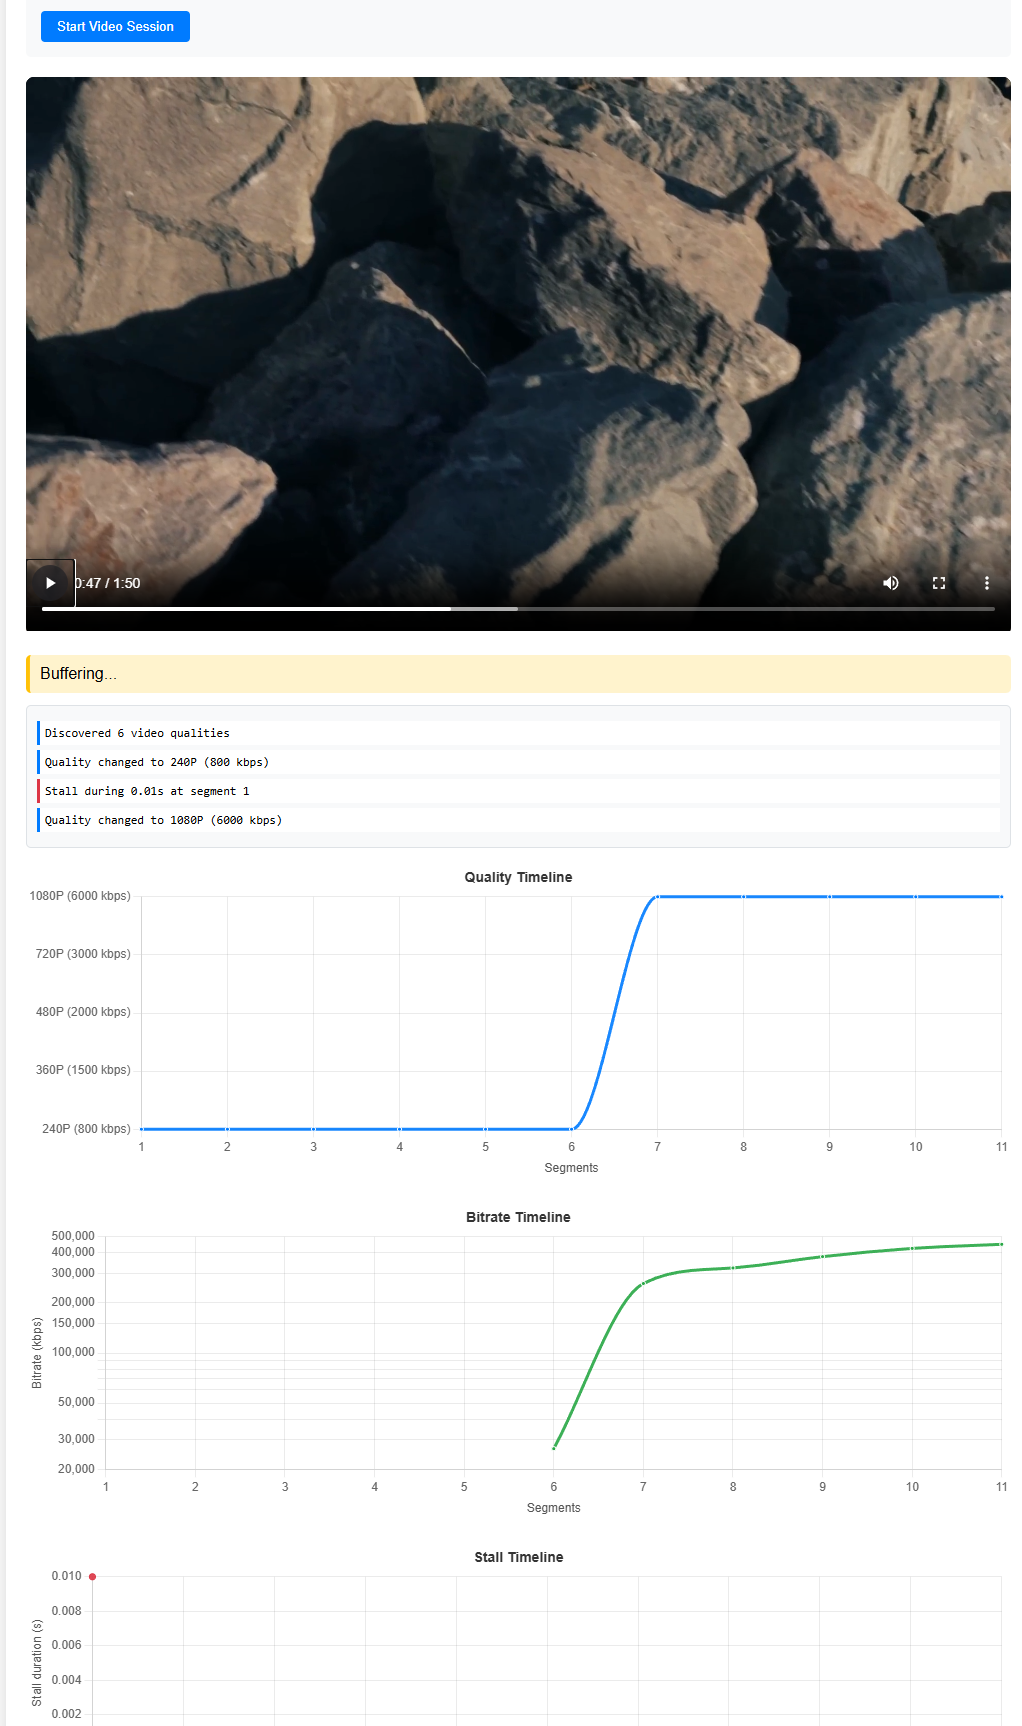
\includegraphics[width=0.83\linewidth]{./Textuais/4-DescricaoExperimento/mpeg-dash-client-charts-and-video.png}
    \text{Fonte: Elaborado pelo autor (2025)}
    \label{fig:dash-client}
\end{figure}

\subsection{Broker MQTT (NanoMQ)}

O \textit{broker} MQTT utilizado no experimento é o NanoMQ, uma implementação leve e de alto desempenho do protocolo MQTT desenvolvida pela EMQ Technologies. O NanoMQ foi escolhido por sua simplicidade de configuração, baixo consumo de recursos e conformidade completa com o padrão MQTT 5.0.

O \textit{broker} é executado em um contêiner Docker dedicado e expõe a porta 1883 para comunicação MQTT não criptografada. A configuração é realizada através de um arquivo \texttt{nanomq.conf} montado como volume no contêiner, permitindo ajustes finos de parâmetros como o número máximo de conexões simultâneas e o tamanho dos \textit{buffers} de mensagens.

No contexto do experimento, o \textit{broker} atua como canal de comunicação entre os servidores MPEG-DASH (publicadores) e o balanceador de carga (assinante), permitindo que as métricas sejam transmitidas de forma assíncrona e desacoplada, sem que os servidores precisem conhecer o endereço do balanceador ou vice-versa.

\subsection{Orquestração com Docker Compose}

A orquestração de todos os componentes do sistema é realizada através do Docker Compose, uma ferramenta para definir e executar aplicações Docker multi-contêiner. O arquivo \texttt{docker-compose.yml} descreve de forma declarativa todos os serviços, suas configurações, limites de recursos, volumes e dependências.

Cada servidor MPEG-DASH é definido como um serviço separado com suas próprias configurações de recursos. Por exemplo, o servidor 1 é configurado com 4096 MB de memória e taxa máxima de leitura de disco de 512 MB/s, enquanto o servidor 8 possui apenas 512 MB de memória e 4 MB/s de leitura de disco. Esta heterogeneidade é fundamental para avaliar a capacidade do algoritmo de balanceamento em distribuir a carga de forma proporcional à capacidade de cada servidor.

Os comandos principais para gerenciar o ambiente experimental são:

\begin{verbatim}
# Limpar cache e iniciar todos os serviços
echo 3 | sudo tee /proc/sys/vm/drop_caches && \
docker compose down && \
docker compose up -d --build

# Visualizar logs do balanceador
docker compose logs -f load-balancer

# Encerrar todos os serviços
docker compose down
\end{verbatim}

\subsection{Painel de Monitoramento}

O painel de monitoramento foi implementado como uma página HTML estática que utiliza a biblioteca Chart.js para renderizar gráficos em tempo real. A página é servida através de um contêiner nginx e se comunica com a API de métricas através de requisições HTTP periódicas utilizando JavaScript.

O painel exibe, para cada servidor e para o balanceador de carga:

\begin{itemize}
    \item Consumo de memória (absoluto e percentual);
    \item Taxa de leitura de disco (MB/s e percentual);
    \item Número de requisições ativas;
    \item Gráficos de séries temporais mostrando a evolução das métricas.
\end{itemize}

O painel é acessível através de um navegador web na porta 3001 do host e foi utilizado durante o desenvolvimento e depuração do sistema para validar o comportamento dos componentes e identificar problemas de configuração. A Figura \ref{fig:monitoring-dashboard} apresenta a interface do painel de monitoramento, mostrando as métricas de múltiplos servidores MPEG-DASH em tempo real.

\begin{figure}[htbp]
    \caption{Painel de monitoramento em tempo real mostrando métricas de consumo de memória, taxa de leitura de disco e requisições ativas dos servidores MPEG-DASH.}
    \centering
    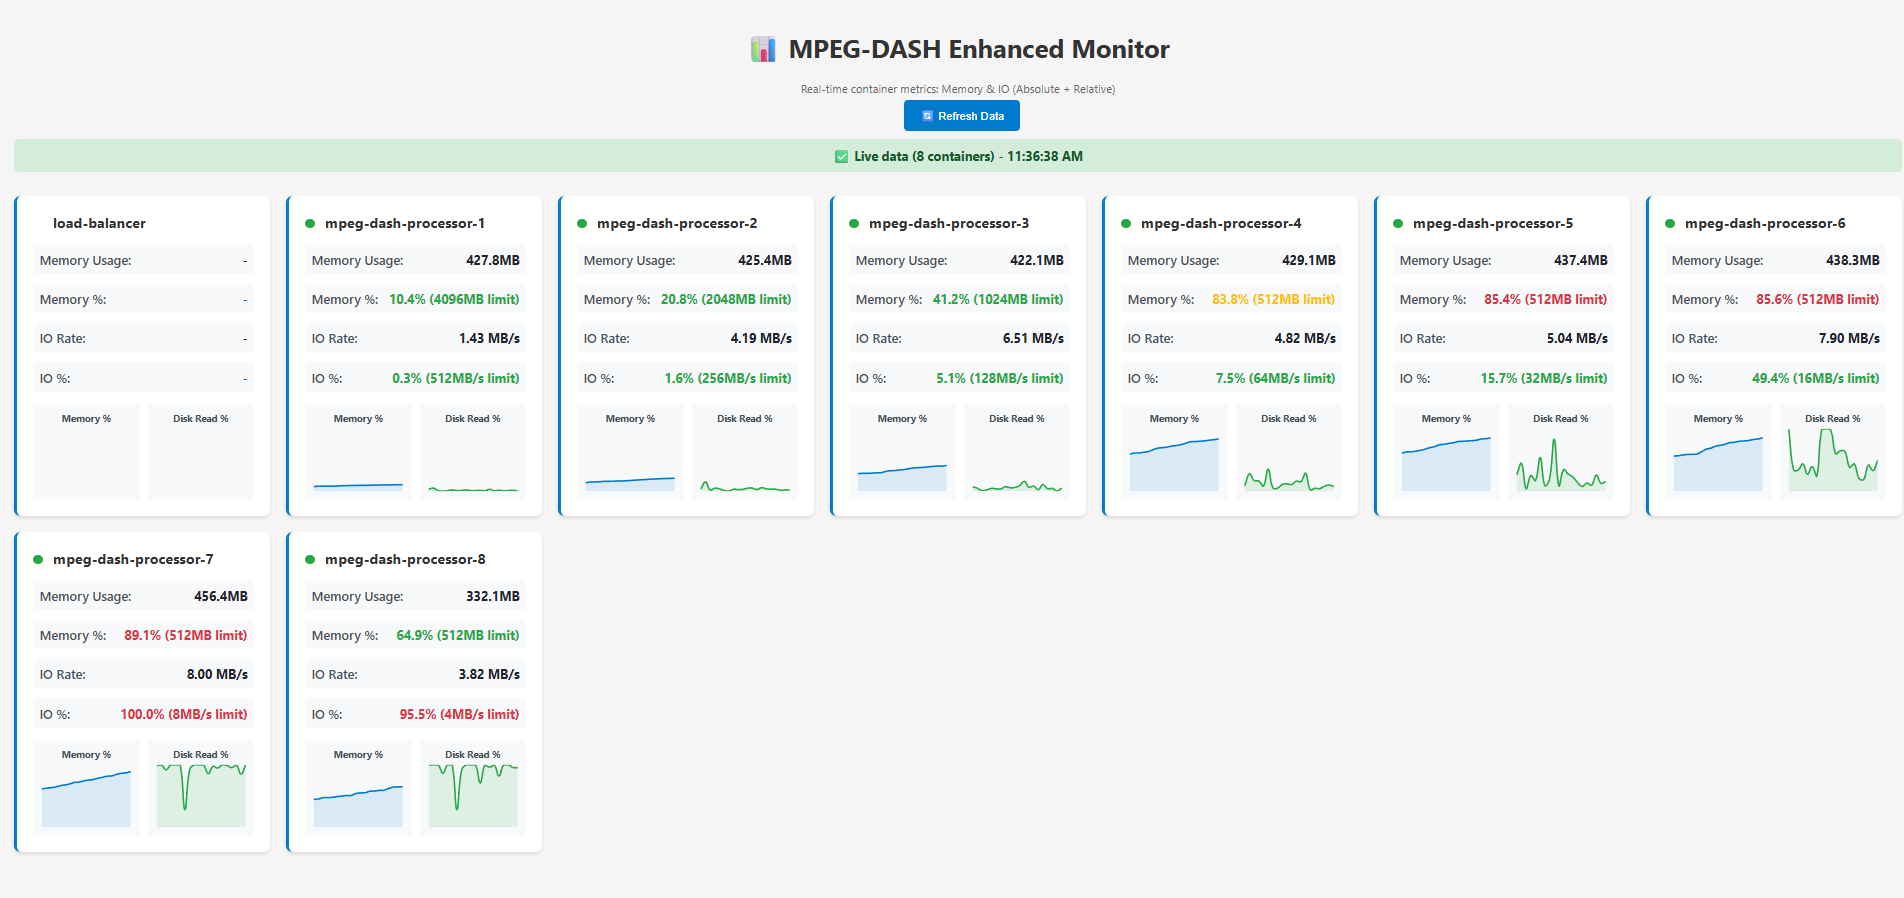
\includegraphics[width=0.95\linewidth]{./Textuais/4-DescricaoExperimento/mpeg-dash-servers-monitoring.png}
    \text{Fonte: Elaborado pelo autor (2025)}
    \label{fig:monitoring-dashboard}
\end{figure}

\section{Geração de Conteúdo}

O conteúdo multimídia utilizado nos experimentos foi gerado utilizando o \texttt{ffmpeg}, uma ferramenta de código aberto amplamente utilizada para processamento de áudio e vídeo. O \texttt{ffmpeg} é capaz de codificar, decodificar, transcodificar, multiplexar e aplicar filtros em arquivos multimídia, sendo a ferramenta padrão da indústria para preparação de conteúdo para \textit{streaming}.

\subsection{Codificação e Segmentação MPEG-DASH}

O processo de geração do conteúdo MPEG-DASH envolveu a conversão de um arquivo de vídeo de entrada para o formato MPEG-DASH com múltiplas representações (resoluções e \textit{bitrates}). O comando utilizado foi:

\begin{verbatim}
ffmpeg -y -i video.mp4 \
-filter_complex "[0:v]format=yuv420p,setsar=1,split=6[v0][v1][v2][v3][v4][v5]; \
                 [v0]scale=1920:1080:flags=lanczos[v1080]; \
                 [v1]scale=1280:720:flags=lanczos[v720]; \
                 [v2]scale=854:480:flags=lanczos[v480]; \
                 [v3]scale=640:360:flags=lanczos[v360]; \
                 [v4]scale=426:240:flags=lanczos[v240]; \
                 [v5]scale=256:144:flags=lanczos[v144]" \
-map "[v1080]" -map "[v720]" -map "[v480]" -map "[v360]" \
     -map "[v240]" -map "[v144]" -map 0:a:0 \
-c:v:0 libx264 -b:v:0 6000k -maxrate:v:0 6600k -bufsize:v:0 12000k \
-c:v:1 libx264 -b:v:1 3000k -maxrate:v:1 3300k -bufsize:v:1 6000k \
-c:v:2 libx264 -b:v:2 2000k -maxrate:v:2 2200k -bufsize:v:2 4000k \
-c:v:3 libx264 -b:v:3 1500k -maxrate:v:3 1650k -bufsize:v:3 3000k \
-c:v:4 libx264 -b:v:4  800k -maxrate:v:4  880k -bufsize:v:4 1600k \
-c:v:5 libx264 -b:v:5  300k -maxrate:v:5  330k -bufsize:v:5  600k \
-profile:v:0 high -profile:v:1 main -profile:v:2 main \
-profile:v:3 main -profile:v:4 main -profile:v:5 main \
-g 120 -keyint_min 120 -sc_threshold 0 -pix_fmt yuv420p \
-preset veryfast \
-c:a aac -b:a 128k -ar 48000 -ac 2 \
-use_template 1 -use_timeline 1 -seg_duration 4 \
-init_seg_name 'init-stream$RepresentationID$.m4s' \
-media_seg_name 'chunk-stream$RepresentationID$-$Number%05d$.m4s' \
-adaptation_sets "id=0,streams=v id=1,streams=a" \
manifest.mpd
\end{verbatim}

Este comando realiza as seguintes operações:

\begin{enumerate}
    \item \textbf{Processamento de Vídeo}: Utiliza um \textit{filter complex} para criar 6 fluxos de vídeo distintos a partir do vídeo de entrada. O filtro \texttt{split} duplica o fluxo de entrada, e cada cópia é redimensionada para uma resolução específica utilizando o algoritmo de escala Lanczos, que oferece alta qualidade visual.
    
    \item \textbf{Resoluções e Bitrates}: São geradas 6 representações de vídeo:
    \begin{itemize}
        \item Full HD (1920×1080) a 6000 kbps
        \item HD (1280×720) a 3000 kbps
        \item 854×480 a 2000 kbps
        \item 640×360 a 1500 kbps
        \item 426×240 a 800 kbps
        \item 256×144 a 300 kbps
    \end{itemize}
    
    \item \textbf{Codificação}: Cada fluxo de vídeo é codificado utilizando o \textit{codec} H.264 (através da biblioteca \texttt{libx264}) com parâmetros específicos de \textit{bitrate} alvo, \textit{bitrate} máximo e tamanho de \textit{buffer}. O perfil H.264 \texttt{high} é utilizado para a resolução Full HD, enquanto o perfil \texttt{main} é usado para as demais resoluções.
    
    \item \textbf{Segmentação}: O vídeo é dividido em segmentos de 4 segundos cada (\texttt{seg\_duration 4}), um valor típico para aplicações de \textit{streaming} adaptativo que oferece um bom equilíbrio entre a granularidade da adaptação e a eficiência de transferência.
    
    \item \textbf{Áudio}: O áudio é codificado em AAC a 128 kbps com taxa de amostragem de 48 kHz e 2 canais (estéreo).
    
    \item \textbf{Manifesto MPD}: É gerado um arquivo \texttt{manifest.mpd} que descreve a estrutura do conteúdo, incluindo as resoluções disponíveis, os \textit{bitrates}, a duração dos segmentos e os \textit{templates} de URL para acessar os arquivos de inicialização e os segmentos de mídia.
\end{enumerate}

\subsection{Replicação e Distribuição do Conteúdo}

Após a geração do conteúdo MPEG-DASH, os arquivos resultantes (manifesto MPD, segmentos de inicialização e segmentos de mídia) foram copiados para um diretório global no sistema de arquivos WSL localizado em \texttt{/data}. Para simular servidores com conteúdo exclusivo, o conteúdo foi replicado em múltiplos subdiretórios utilizando o comando \texttt{rsync}:

\begin{verbatim}
sudo rsync -a --progress ./server-1/ ./server-2/
sudo rsync -a --progress ./server-1/ ./server-3/
# ... continuando até server-8
\end{verbatim}

Cada subdiretório \texttt{/data/server-X} foi então montado como um volume no contêiner correspondente através da diretiva \texttt{volumes} no arquivo \texttt{docker-compose.yml}:

\begin{verbatim}
volumes:
  - /data/server-1:/app/wwwroot/Static
\end{verbatim}

Este mecanismo de \textit{bind mount} permite que cada servidor acesse apenas seu próprio conjunto de arquivos, simulando o cenário realista de uma CDN onde cada servidor de borda mantém uma cópia local do conteúdo. A utilização de \textit{bind mounts} também facilita a atualização do conteúdo sem necessidade de reconstruir as imagens Docker, uma vez que as modificações no diretório do host são imediatamente refletidas dentro dos contêineres.

\section{Cenários de Teste}

A avaliação experimental do algoritmo proposto foi conduzida através de múltiplos cenários de teste, projetados para avaliar o desempenho do sistema sob diferentes condições de carga e configurações de recursos dos servidores. Os cenários foram cuidadosamente definidos para permitir uma análise comparativa rigorosa entre as diferentes estratégias de balanceamento de carga.

\subsection{Parâmetros Globais}

Todos os cenários de teste compartilham os seguintes parâmetros:

\begin{itemize}
    \item \textbf{\textit{Timeout} de requisição}: 30 segundos
    \item \textbf{Número de vídeos no catálogo}: 12
    \item \textbf{Número de resoluções disponíveis}: 6 (conforme descrito na seção anterior)
\end{itemize}

\subsection{Definição dos Cenários}

Foram definidos quatro cenários principais, cada um testado com três estratégias de balanceamento diferentes (Round-Robin, Seleção Aleatória e Monitoramento de Memória com diferentes intervalos de atualização). A Tabela \ref{tab:test-scenarios} apresenta a especificação detalhada de cada cenário.

\begin{table}[htbp]
\centering
\caption{Cenários de teste definidos para avaliação experimental}
\label{tab:test-scenarios}
\small
\begin{tabular}{|c|c|c|p{6.5cm}|}
\hline
\textbf{Cenário} & \textbf{Usuários} & \textbf{Distribuição} & \textbf{Configuração dos Servidores} \\
\hline
1 & 100 & Heterogênea & 
\textbf{S1}: 4096MB / 512MB/s; \newline
\textbf{S2}: 2048MB / 256MB/s; \newline
\textbf{S3}: 1024MB / 128MB/s; \newline
\textbf{S4}: 512MB / 64MB/s; \newline
\textbf{S5}: 512MB / 32MB/s; \newline
\textbf{S6}: 512MB / 16MB/s; \newline
\textbf{S7}: 512MB / 8MB/s; \newline
\textbf{S8}: 512MB / 4MB/s \\
\hline
2 & 100 & Homogênea & 
Todos os servidores: 1024MB RAM e 256MB/s I/O \\
\hline
3 & 1000 & Heterogênea & 
Mesma configuração do Cenário 1 \\
\hline
4 & 1000 & Homogênea & 
Mesma configuração do Cenário 2 \\
\hline
\end{tabular}
\end{table}

\subsection{Descrição dos Cenários}

\subsubsection{Cenário 1: Baixa Concorrência com Servidores Heterogêneos}

Este cenário simula uma situação de carga moderada com 100 usuários simultâneos acessando um conjunto de servidores com capacidades significativamente diferentes. A heterogeneidade dos recursos visa avaliar a capacidade do algoritmo proposto de identificar e priorizar servidores com maior disponibilidade de recursos. Espera-se que estratégias que ignoram o estado dos servidores (como Round-Robin e Seleção Aleatória) distribuam a carga de forma uniforme, potencialmente sobrecarregando os servidores menos capazes, enquanto o algoritmo de monitoramento de memória deve ser capaz de direcionar mais requisições para os servidores com maior capacidade.

\subsubsection{Cenário 2: Baixa Concorrência com Servidores Homogêneos}

Este cenário mantém o mesmo nível de carga do Cenário 1, mas utiliza servidores com recursos idênticos. O objetivo é avaliar o comportamento das estratégias em um ambiente onde não há vantagem teórica em favorecer um servidor específico. Neste cenário, espera-se que todas as estratégias apresentem desempenho similar, uma vez que a distribuição uniforme de carga é adequada quando os servidores possuem capacidades equivalentes.

\subsubsection{Cenário 3: Alta Concorrência com Servidores Heterogêneos}

Este cenário eleva significativamente a carga do sistema para 1000 usuários simultâneos, mantendo a configuração heterogênea de servidores. O objetivo é avaliar o comportamento das estratégias sob condições de alta pressão, onde a capacidade de identificar e evitar servidores sobrecarregados torna-se crítica para manter a qualidade de serviço. Este é o cenário mais exigente e onde se espera observar as maiores diferenças de desempenho entre as estratégias.

\subsubsection{Cenário 4: Alta Concorrência com Servidores Homogêneos}

O último cenário combina alta carga com servidores homogêneos, oferecendo um ponto de comparação para o Cenário 3. Ele permite avaliar se as diferenças observadas no Cenário 3 são devidas à heterogeneidade dos recursos ou ao nível de carga do sistema.

\subsection{Estratégias de Balanceamento Avaliadas}

Para cada um dos quatro cenários descritos, foram executados testes com as seguintes estratégias de balanceamento:

\begin{enumerate}
    \item \textbf{Round-Robin}: Estratégia de linha de base que distribui as requisições de forma cíclica entre os servidores.
    
    \item \textbf{Seleção Aleatória}: Estratégia de linha de base que seleciona um servidor aleatoriamente para cada requisição.
    
    \item \textbf{Monitoramento de Memória (intervalo médio de 6 segundos)}: Algoritmo proposto com intervalo médio de atualização de métricas de 6 segundos, representando um cenário com informações relativamente atualizadas.
    
    \item \textbf{Monitoramento de Memória (intervalo médio de 30 segundos)}: Algoritmo proposto com intervalo médio de atualização de 30 segundos, representando um cenário com informações moderadamente desatualizadas.
\end{enumerate}

Cada combinação de cenário e estratégia de balanceamento foi implementada como uma \textit{branch} Git específica no repositório do projeto, permitindo o isolamento e a reprodutibilidade de cada configuração experimental. Esta organização através de \textit{branches} facilitou a execução sistemática dos testes e garantiu que as diferentes configurações não interferissem entre si.

A avaliação com diferentes intervalos de atualização visa demonstrar a robustez do algoritmo proposto mesmo quando operando com informações de carga moderadamente obsoletas, uma situação comum em sistemas distribuídos de larga escala onde o custo de monitoramento muito frequente pode ser proibitivo.

\subsection{Métricas de Avaliação}

Para cada combinação de cenário e estratégia de balanceamento, foram coletadas as seguintes métricas de Qualidade de Experiência (QoE):

\begin{itemize}
    \item Número total de travamentos (\textit{stalls}) observados durante a reprodução do vídeo;
    \item Duração média de cada travamento em milissegundos;
    \item Tempo total de ociosidade (soma de todas as pausas) em segundos;
    \item Taxa de erros de requisições HTTP (percentual de requisições que falharam);
    \item Latência média de resposta das requisições em milissegundos.
\end{itemize}

Estas métricas foram escolhidas por seu impacto direto na experiência percebida pelo usuário final ao consumir conteúdo de vídeo em \textit{streaming}. A análise comparativa destas métricas entre as diferentes estratégias permite quantificar objetivamente o benefício (ou eventual desvantagem) do algoritmo proposto em relação às abordagens convencionais.

